\section{Simulation study}\label{sec:simulation}

\subsection{Design}\label{sec:sim-design}

The study follows \citet{morris2019} and addresses hypotheses H1 to H3.

\paragraph{Data-generating mechanisms.} Every evaluation of alternative $k$ is a vector whose components have Beta distributions with means $\mu_{k,i}$ and concentration $\kappa$ (variance $\mu_{k,i}(1-\mu_{k,i})/(\kappa+1)$), coupled through a Gaussian copula with correlation $\rho$ between every pair of objectives. Study~1 uses six fixed configurations in which a wrong statement is easy to make: \emph{flat}, four Pareto-optimal alternatives with $m=2$, two of them closer than $\varepsilon=0.02$; \emph{close}, an alternative dominated by $0.03$ in both objectives next to three Pareto-optimal ones, $\varepsilon=0.02$, so that both a false discard and a false acceptance are possible; \emph{boundary}, an alternative dominated by exactly $\varepsilon=0.02$ in both objectives, which may be discarded but never accepted, next to three Pareto-optimal ones; \emph{cycle}, \emph{ties} and \emph{chain}, the instances of Proposition~\ref{prop:failure}(a), (b) and (c) with $\varepsilon=0.1$. The concentration is $\kappa=20$ in the first three and $\kappa=200$ in the last three. Study~2 draws a new instance in every replication: about half of the $K$ alternatives lie on the linear front $\sum_i\mu_{k,i}=\text{const}$ inside $[0.2,0.8]^m$, at points drawn uniformly on the simplex, and each of the others is a front point shifted upward by independent $U(0.02,0.15)$ amounts in every objective. The main grid crosses $K\in\{5,10,20\}$ with $\varepsilon\in\{0.025,0.05,0.10\}$ for $m=2$, $\kappa=20$ and $\rho=0$; secondary cells set $K=10$ and $\varepsilon=0.05$ and vary $m=3$, $\rho=\pm0.6$, or the confidence sequence.

\paragraph{Methods.} All methods use $\alpha=0.05$, an initial batch of $n_0=5$ evaluations per alternative and batches of $b=5$. The proposed procedure (Algorithm~\ref{alg:procedure}, betting sequences on a grid of 1001 points without endpoint refinement) is compared with three variants that each change one ingredient: $\varepsilon$-elimination with the tie-break and the allocation of our first implementation (``$\varepsilon$-discarding''); fixed-sample Student-$t$ intervals recomputed after every batch, at the same split level $\alpha/(Km)$ (``repeated $t$''); and betting sequences at level $\alpha$ each, without the union bound (``no correction''). Study~2 also compares the open-pair allocation with uniform allocation, which evaluates every plausible alternative in turn. The budget is $10^4$ evaluations in Study~1 and $3\times10^4$ in Study~2.

\paragraph{Performance measures.} After every batch, every statement of Theorem~\ref{thm:validity} is checked against the true means: a discarded alternative that is not dominated, an accepted alternative outside $\Peps$, a certified-optimal alternative outside $\Pset$, and, at the end, representatives that fail to $\epsb$-cover $\Pset$. A replication counts as an \emph{error} if any of these occurs at any time. For $\varepsilon$-discarding the corresponding statement is that each discarded alternative is truly $\epsb$-dominated. For all methods we record \emph{frontier loss}, the event that the plausible set fails to $\epsb$-cover $\Pset$ at some time, which is the common target of all methods. We also record the number of evaluations and whether the identification ended before the budget. Study~1 uses 200 replications per cell, so that an error rate of $0.05$ is estimated with a Monte Carlo standard error of about $0.015$; Study~2 uses 30 replications per cell.

\subsection{Results}\label{sec:sim-results}

\paragraph{Validity (Study~1).} Table~\ref{tab:validity} reports, for each configuration and method, the percentage of replications with an error and with frontier loss and the median number of evaluations. The proposed procedure made no false statement in any of the 1200 replications and always stopped. $\varepsilon$-discarding lost the Pareto set in every replication of the cycle configuration and in 1.5\% of the chain configuration. In the tie configuration it lost nothing: the certificates $2\to1$ and $3\to2$ have larger margins than the ties of Proposition~\ref{prop:failure}(b) and appear first, so alternative~3 survives alone and covers the other two. Its allocation, which evaluates only undecided alternatives, did not stop within $10^4$ evaluations in the flat, close and chain configurations, the stalling discussed in Section~\ref{sec:allocation}. Repeated $t$ intervals stopped earliest and were the only method to err, in 3.5\% of the replications of the close configuration (95\% Clopper--Pearson interval 1.4\% to 7.1\%); this rate is below the nominal level, and the configurations were not adverse enough to push it above. In the boundary configuration no method erred, and the proposed procedure needed a median of 4982 evaluations, against 1555 for repeated $t$ intervals and 3322 without the union bound, which is the price of validity in this configuration. Confidence sequences without the union bound made no error, which we discuss in Section~\ref{sec:discussion}.

\begin{table}[tbp]
\spacingset{1}
\centering
\caption{Study~1: percentage of the 200 replications with an error (Err.) and with frontier loss (Loss), and median number of evaluations (Eval.); in parentheses, the percentage that stopped within $10^4$ evaluations when below 100. With 200 replications, the upper 95\% Clopper--Pearson limit for an observed rate of zero is 1.8\%.}
\label{tab:validity}
\footnotesize
\begin{tabular}{llrrrr}
\toprule
Configuration & Method & Error (\%) & Frontier loss (\%) & Stopped (\%) & Evaluations \\
\midrule
flat & proposed & 0.0 (0.0, 1.8) & 0.0 (0.0, 1.8) & 100 & 1390 \\
 & $\varepsilon$-discarding & 0.0 (0.0, 1.8) & 0.0 (0.0, 1.8) & 0 & 10000 \\
 & repeated $t$ & 0.0 (0.0, 1.8) & 0.0 (0.0, 1.8) & 100 & 532 \\
 & no correction & 0.0 (0.0, 1.8) & 0.0 (0.0, 1.8) & 100 & 935 \\
\addlinespace
close & proposed & 0.0 (0.0, 1.8) & 0.0 (0.0, 1.8) & 100 & 3268 \\
 & $\varepsilon$-discarding & 0.0 (0.0, 1.8) & 0.0 (0.0, 1.8) & 0 & 10000 \\
 & repeated $t$ & 3.5 (1.4, 7.1) & 0.5 (0.0, 2.8) & 100 & 1260 \\
 & no correction & 0.0 (0.0, 1.8) & 0.0 (0.0, 1.8) & 100 & 2185 \\
\addlinespace
boundary & proposed & 0.0 (0.0, 1.8) & 0.0 (0.0, 1.8) & 99 & 4982 \\
 & $\varepsilon$-discarding & 0.0 (0.0, 1.8) & 0.0 (0.0, 1.8) & 100 & 1390 \\
 & repeated $t$ & 0.0 (0.0, 1.8) & 0.0 (0.0, 1.8) & 100 & 1555 \\
 & no correction & 0.0 (0.0, 1.8) & 0.0 (0.0, 1.8) & 100 & 3322 \\
\addlinespace
cycle & proposed & 0.0 (0.0, 1.8) & 0.0 (0.0, 1.8) & 100 & 225 \\
 & $\varepsilon$-discarding & 0.0 (0.0, 1.8) & 100.0 (98.2, 100.0) & 100 & 730 \\
 & repeated $t$ & 0.0 (0.0, 1.8) & 0.0 (0.0, 1.8) & 100 & 20 \\
 & no correction & 0.0 (0.0, 1.8) & 0.0 (0.0, 1.8) & 100 & 145 \\
\addlinespace
ties & proposed & 0.0 (0.0, 1.8) & 0.0 (0.0, 1.8) & 100 & 230 \\
 & $\varepsilon$-discarding & 0.0 (0.0, 1.8) & 0.0 (0.0, 1.8) & 100 & 545 \\
 & repeated $t$ & 0.0 (0.0, 1.8) & 0.0 (0.0, 1.8) & 100 & 20 \\
 & no correction & 0.0 (0.0, 1.8) & 0.0 (0.0, 1.8) & 100 & 155 \\
\addlinespace
chain & proposed & 0.0 (0.0, 1.8) & 0.0 (0.0, 1.8) & 100 & 230 \\
 & $\varepsilon$-discarding & 0.0 (0.0, 1.8) & 1.5 (0.3, 4.3) & 2 & 10000 \\
 & repeated $t$ & 0.0 (0.0, 1.8) & 0.0 (0.0, 1.8) & 100 & 20 \\
 & no correction & 0.0 (0.0, 1.8) & 0.0 (0.0, 1.8) & 100 & 150 \\
\bottomrule
\end{tabular}

\end{table}

\paragraph{Efficiency (Study~2).} No method made a false statement in Study~2 (Figure~\ref{fig:efficiency}). The open-pair allocation needed fewer evaluations than uniform allocation in every cell of the main grid, with median savings between 18\% and 44\%; the saving was largest for $\varepsilon=0.05$ and smallest for $\varepsilon=0.10$, and it did not increase with $K$. The number of evaluations grew faster than in proportion to $K$ and much less than in proportion to $\varepsilon^{-2}$. $\varepsilon$-discarding with its own allocation stopped in a proportion of replications that fell with $K$ and with smaller tolerances, and with $K=20$ and $\varepsilon=0.10$ it lost part of the Pareto set in 43\% of the replications. In the secondary cells, three objectives raised the median from 3613 to 5018 evaluations (7835 with uniform allocation), correlations of $\pm0.6$ raised it to about 4000, the empirical-Bernstein sequence needed 6455, and the Hoeffding sequence did not stop within $3\times10^4$ evaluations in any replication. Table~\ref{S-tab:study2} of the Supplementary Material gives all cells.

\begin{figure}[t]
\spacingset{1}
\centering
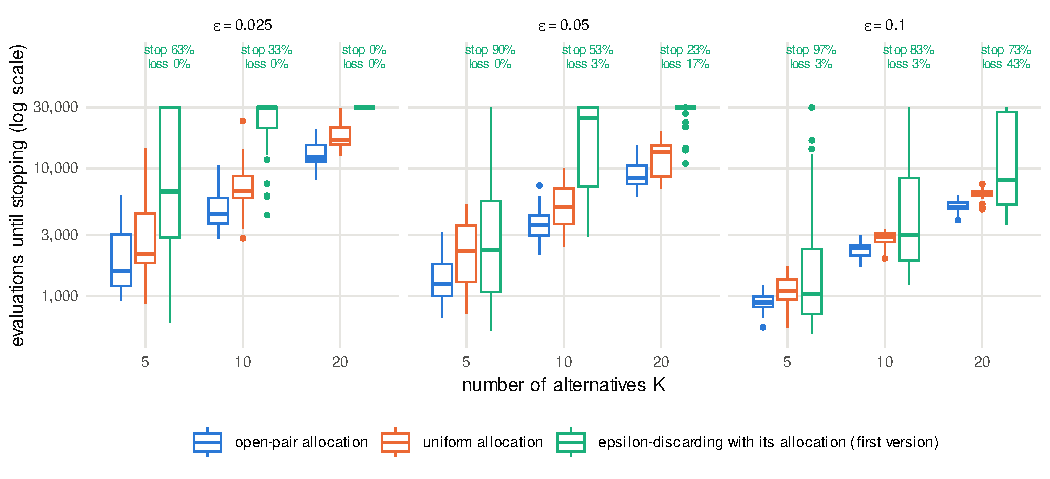
\includegraphics[width=0.92\textwidth]{figures/fig2_efficiency.pdf}
\caption{Study~2: number of evaluations until stopping, 30 random instances per box, $m=2$, $\rho=0$. Boxes for $\varepsilon$-discarding include replications censored at $3\times10^4$; the labels give the percentage that stopped and the percentage with frontier loss.}
\label{fig:efficiency}
\end{figure}

